\section{Segunda consigna: gráficos y análisis}

\subsection{Red con información previa}
Aquí irá la red tomada de alguna casa, oficina, o algo que sepamos algo...--------------

\subsection{Redes sin información previa}
A continuación se muestra la cantidad de paquetes ARP por host en escala logarítmica. 
En el momento de realizar los gráficos, notamos que contabamos con una gran cantidad de hosts con muy baja probabilidad. 
Para mejorar la claridad y permitir apreciar los resultados a gran escala, decidimos filtrar estos casos y expresarlos como $Otros$ ya que 
no vimos valor en mostrar nodos con un 0,05 de probabilidad.\\

\subsubsection{Red Wifi: laboratorioDC}
\begin{figure}[h!]
\centering
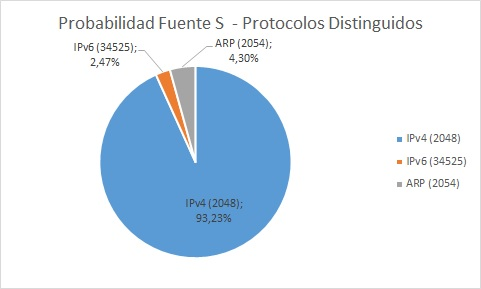
\includegraphics[width=\textwidth]{./img/probaS_laboDC.jpg}
\caption{Protocolos Distinguidos - Fuente S - laboratoriosDC}
\end{figure}
\newpage

\begin{figure}[h!]
\centering
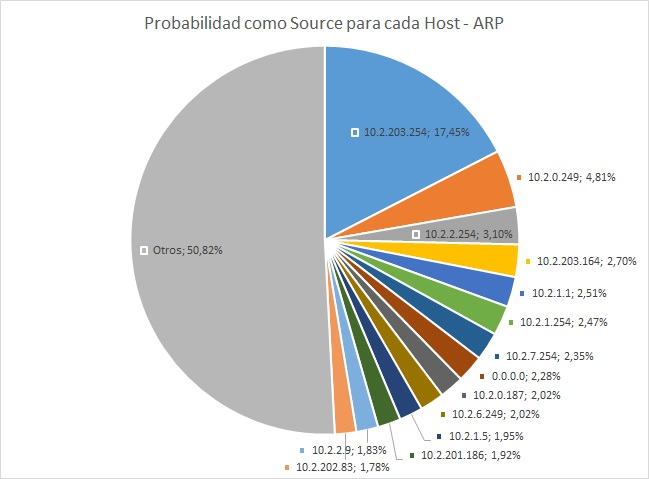
\includegraphics[width=\textwidth]{./img/proba_src_laboDC.jpg}
\caption{Probabilidad Source - Fuente S1(ARP) - laboratoriosDC}
\end{figure}

\begin{figure}[h!]
\centering
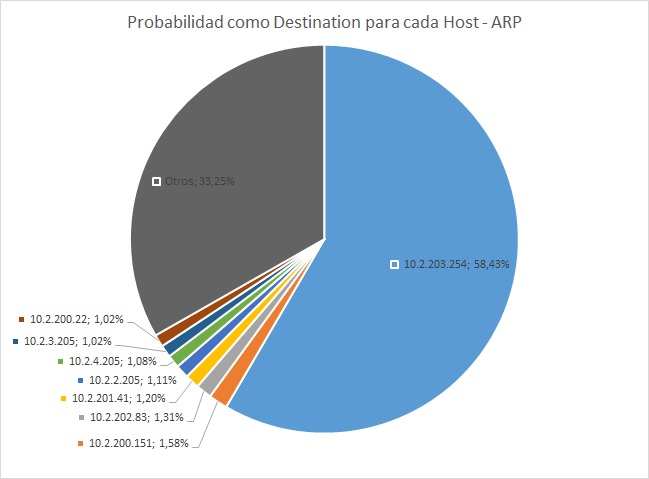
\includegraphics[width=\textwidth]{./img/proba_dst_laboDC.jpg}
\caption{Probabilidad Destination - Fuente S1(ARP) - laboratoriosDC}
\end{figure}
\newpage

\begin{figure}[h!]
\centering
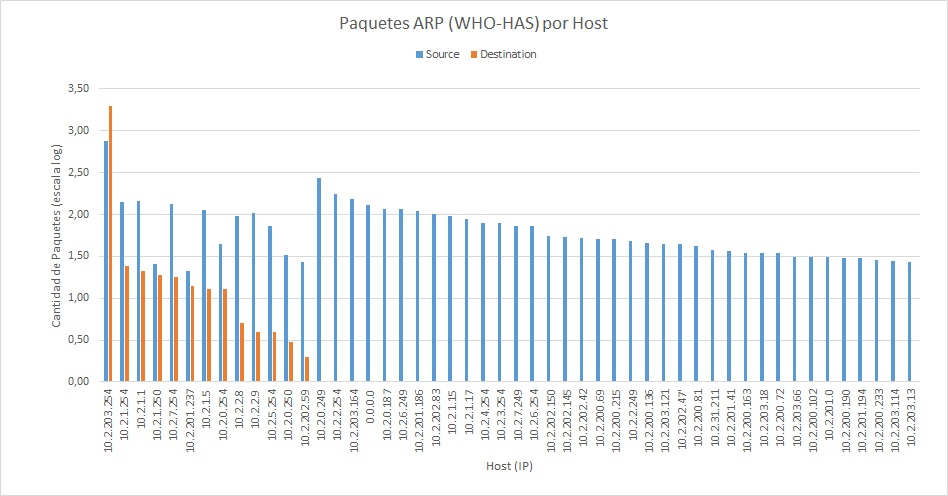
\includegraphics[width=\textwidth]{./img/arp_whoHas_laboDC.jpg}
\caption{Source/Destination paquetes ARP - Operación: Who-Has - laboratoriosDC}
\end{figure}

\begin{figure}[h!]
\centering
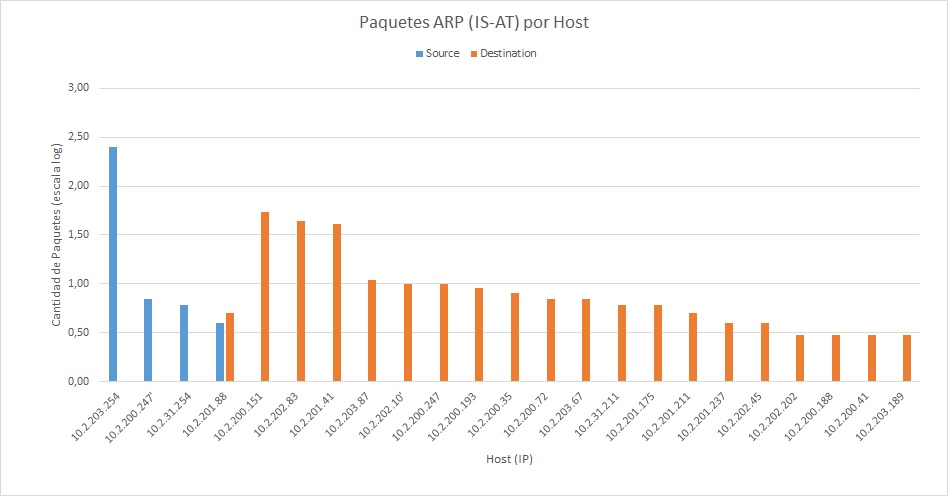
\includegraphics[width=\textwidth]{./img/arp_isAt_laboDC.jpg}
\caption{Source/Destination paquetes ARP - Operación: Is-At - laboratoriosDC}
\end{figure}


\newpage
\subsubsection{Red Wifi: aulasDC}
\begin{figure}[h!]
\centering
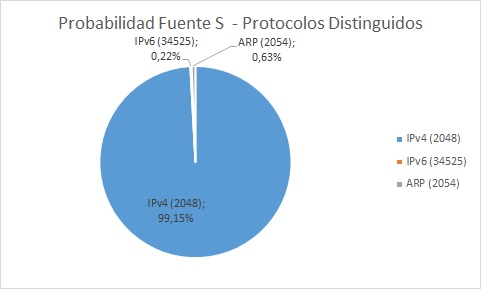
\includegraphics[width=\textwidth]{./img/probaS_aulasDC.jpg}
\caption{Protocolos Distinguidos - Fuente S - aulasDC}
\end{figure}
\newpage

\begin{figure}[h!]
\centering
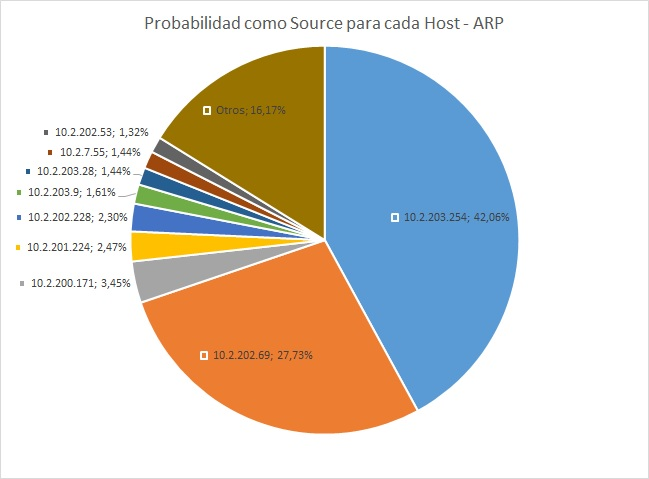
\includegraphics[width=\textwidth]{./img/proba_src_aulasDC.jpg}
\caption{Probabilidad Source - Fuente S1(ARP) - aulasDC}
\end{figure}

\begin{figure}[h!]
\centering
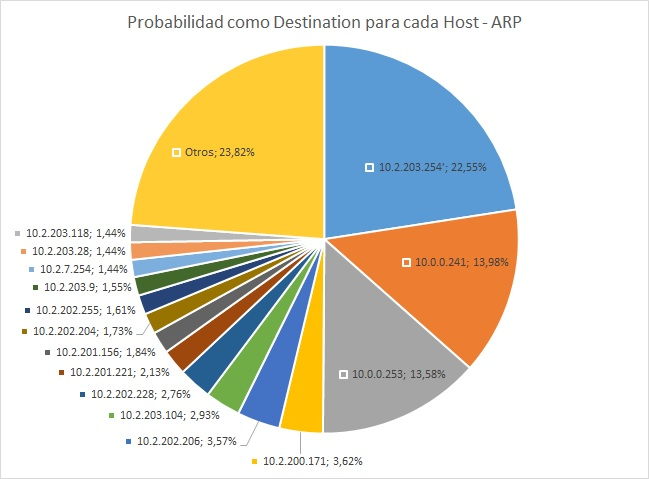
\includegraphics[width=\textwidth]{./img/proba_dst_aulasDC.jpg}
\caption{Probabilidad Destination - Fuente S1(ARP) - aulasDC}
\end{figure}
\newpage

\begin{figure}[h!]
\centering
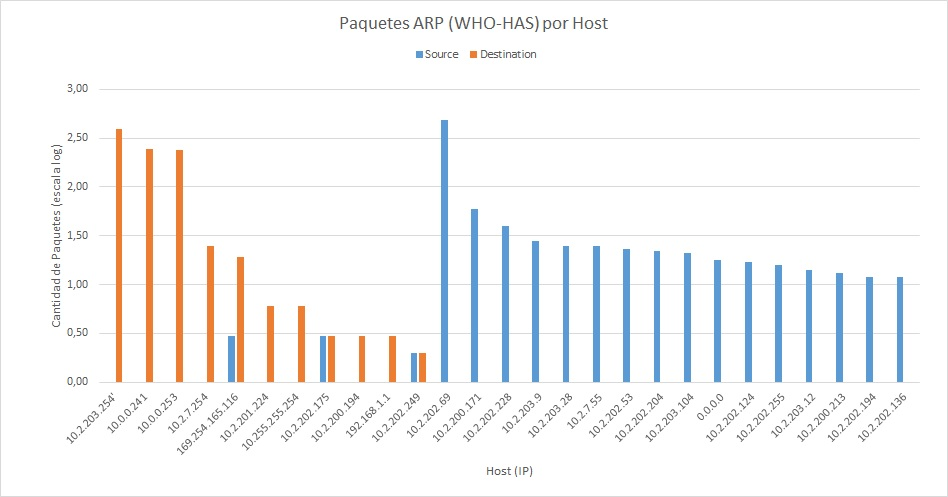
\includegraphics[width=\textwidth]{./img/arp_whoHas_aulasDC.jpg}
\caption{Source/Destination paquetes ARP - Operación: Who-Has - aulasDC}
\end{figure}

\begin{figure}[h!]
\centering
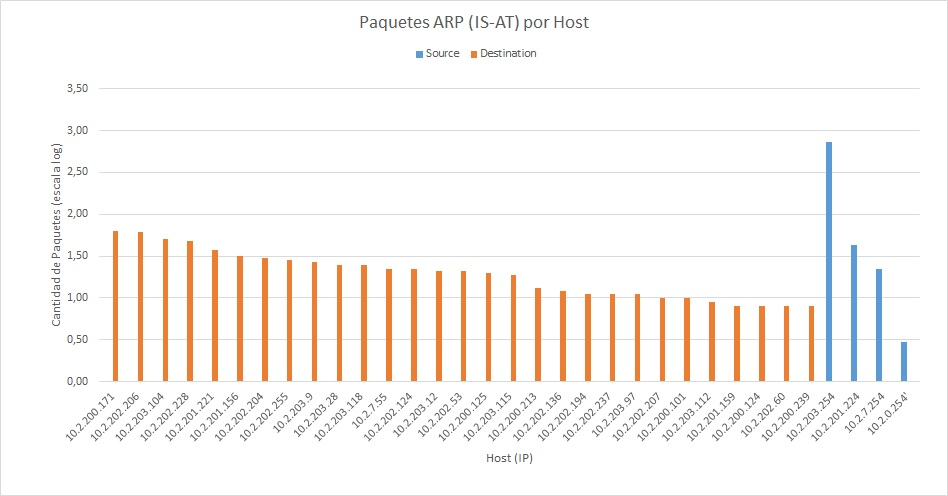
\includegraphics[width=\textwidth]{./img/arp_isAt_aulasDC.jpg}
\caption{Source/Destination paquetes ARP - Operación: Is-At - aulasDC}
\end{figure}


\newpage
\subsubsection{Red Wifi: A DEFINIR}